% !TeX encoding = UTF-8
% !TeX root = ../main.tex
\chapter{Implementácia vzorovej sady grafických komponentov}

\section{Vzorová sada}
Vzorová sada grafických komponentov SCADA systémov obsahuje:
\begin{itemize}
	\item Thermometer - obrázok \ref{fig:thermometer}
	\item Trojcestný ventil - obrázok \ref{fig:trippleValve}
	\item Mapa Slovenska - obrázok \ref{fig:map}
	\item Prečerpávacia stanica - obrázok \ref{fig:pump}
	\item Prepravný pás - obrázok \ref{fig:belt}
	
\end{itemize}
%%%%%%%%%%%%%%%%%%%%%%%
\begin{figure}[H]
	\centering
	
\includegraphics{obrazky/thermometer}
	\caption{Termometer}
	\label{fig:thermometer}
\end{figure}
%%%%%%%%%%%%%%%%%%%%%%%%%%%%%%%%%
\begin{figure}[H]
	\centering
	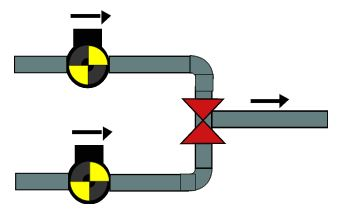
\includegraphics[width=0.7\linewidth]{obrazky/trippleValve}
	\caption{Trojcestný ventil}
	\label{fig:trippleValve}
\end{figure}
%%%%%%%%%%%%%%%%%%%%%%%%%%%%%%%%%%%%%%%%%
\begin{figure}[H]
	\centering
	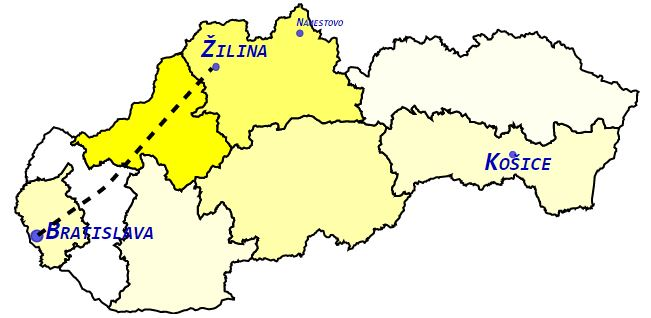
\includegraphics[width=0.7\linewidth]{obrazky/map}
	\caption{Mapa Slovenska}
	\label{fig:map}
\end{figure}
%%%%%%%%%%%%%%%%%%%%%%%%%%%%%%%%%%%%%%%%%%

\begin{figure}[H]
	\centering
	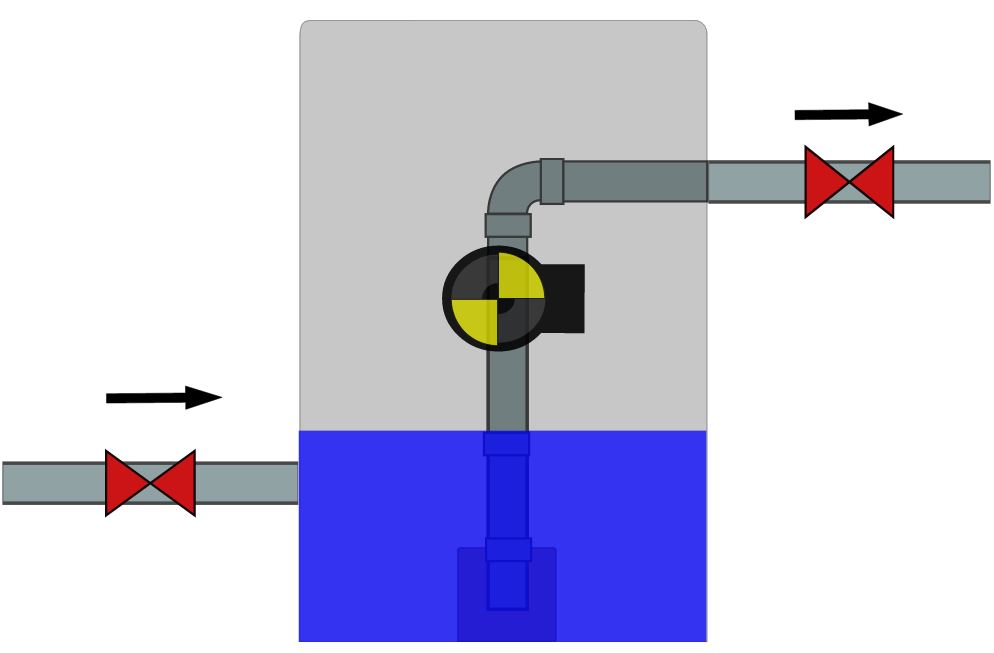
\includegraphics[width=0.7\linewidth]{obrazky/pump}
	\caption{Prečerpávacia stanica}
	\label{fig:pump}
\end{figure}
%%%%%%%%%%%%%%%%%%%%%%%%%%%%%%%%%%%%%%%%%%%%%%%%%%%
\begin{figure}[H]
	\centering
	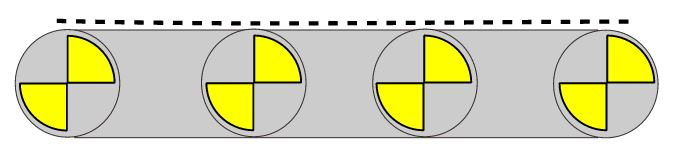
\includegraphics[width=0.7\linewidth]{obrazky/belt}
	\caption{Prepravný pás}
	\label{fig:belt}
\end{figure}
%%%%%%%%%%%%%%%%%%%%%%%%%%%%%%%%%%%%%%%%%%%%


\section{Príklad vytvorenia prečerpávacej stanice v Inkscape}

Nakreslenie jednotlivých častí komponentov prečerpávacej stanice v Inkscape bolo realizované pomocou ľavého bočného panela. Prečerpávacia stanica sa skladá z potrubí, indikátora úrovne hladiny vody, motora, a dvoch symbolov prítoku hladiny. Ako je možné vidieť na obrázku  \ref{picture1}.  


\begin{figure}[H]
	\begin{center}
		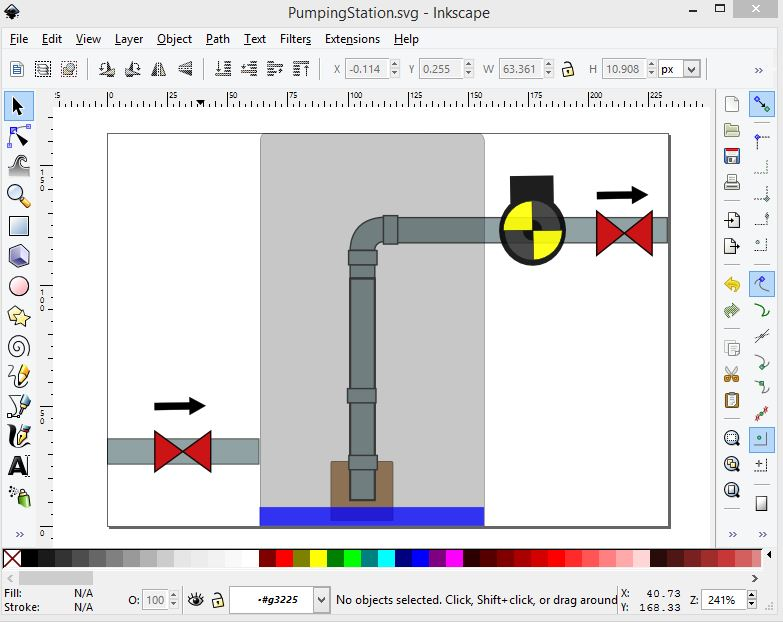
\includegraphics[width=0.7\linewidth] {obrazky/pump1.jpg}
		\caption{Grafické prostredie programu Inkscape s nakreslenou prečerpávacou stanicou}
		\label{picture1}
	\end{center}
\end{figure}


\section{Definovanie id v SVG}

Pre ovládanie JavaScriptom je nutné si pozrieť jednotlivé jedinečné identifikačné názvy. V SVG sú označované ako id. V zdrojovom kóde .svg súboru je to označené id="nazovElementu". Na ovládanie časti svg elementu v JavaScripte bude realizované cez CSS selektor, kde pristúpim k id svg cez značku \#. 
Príklad použitia: paper.select("\#ventil"); .


\subsection{Object Properties}
Zistenie id je pomerne jednoduché v Inkscape. Klikneme pravým tlačidlom na daný komponent, ktorého id chceme vedieť, a potom na Objekt Properties.

Po kliknutí sa nám zobrazí okno s názvom Object Properties. 

\begin{figure}[H]
	\begin{center}
		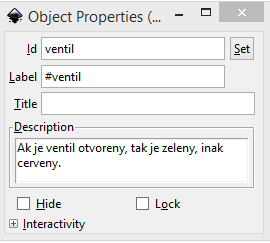
\includegraphics [width=5cm]  {obrazky/obr3.png}
		\caption{Object Properties}
		\label{picture3}
	\end{center}
\end{figure}


Z obrázka č.\ref{picture3} možno vyčítať aké je ID, predvolené sú tam napríklad desc3072. Hodnoty je možné prepísať a zmeniť stlačením tlačidla Set. Pre nás je dôležitá hodnota v kolónke id - ventil. 

V okne Object Properties je možné nastaviť script na animovanie. Po kliknutí na Interactivity sa zobrazia ďalšie kolónky, kde je možné zadať akciu, ktorá má nastať.  


\subsection{XML Editor}
Ďalší spôsob získania informácii o svg cez Inkscape je cez zabudovaný XML Editor.
Stlačením klávesovej skratky SHIFT + CTRL + X, alebo v hornej lište v menu vybrať ponuku Edit a na spodku je XML Editor. Následne sa zobrazí okno, ktoré je na obrázku \ref{xmlEditor}.
\begin{figure}[H]
	\begin{center}
		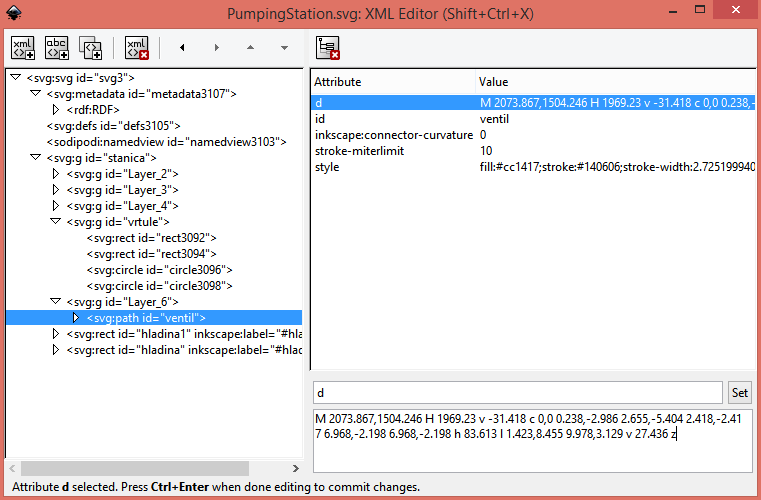
\includegraphics[width=0.6\linewidth]  {obrazky/XmlEditor2.png}
		\caption{Xml Editor v Inkscape}
		\label{xmlEditor}
	\end{center}
\end{figure}

XML Editor umožní zistiť ID jednotlivých komponentov, ale i hodnoty atribútov. 


\section{Integrácia prečerpávacej stanice pre dynamické ovládanie SVG objektu}

Súborová štruktúra prečerpávacej stanice: 
\begin{itemize}
	\item index.html 
	\item PumpingStation.js
	\item PumpingStation.svg
	\item TestPumpingStation.js
\end{itemize}

\subsection{HTML súbor}
Do HTML súboru index.html pridáme párový tag $<$svg$>$.  Na toto miesto sa neskôr vykreslí SVG načítané zo súboru cez JavaScript. Môže sa tu uviesť i celý kód SVG obrázka. V prípade, že nebude v dokumente dané kde presne sa nachádza SVG tag tak sa pridá na najbližšie voľné miesto. 
\subsection{Kód}
\begin{lstlisting}
<svg 
	id="svgStanica" 
	viewBox="0 0 750 600" 
	width="40%" 
	height="40%"> 
</svg>
\end{lstlisting}

\subsection{Vysvetlenie kódu}
Atribúty v tagu sú prispôsobené na to, aby sa grafický element vykreslil responzívne na obrazovku.
\begin{itemize}
\item  \textbf{id} - jedinečný identifikátor, cez ktorý meníme vlastnosti.
\item 	\textbf{viewBox} - je virtuálne okno, ktorým sa užívateľ uvidí svg obrázok. Je atribút, ktorý povoľuje špecifikovať danú množinu grafických komponentov, aby sa zobrazili v daných súradniciach x, y a šírke, výške. Hodnoty atribútov v viewBox sú štyri čísla - min-x, min-y, width a height. 
\item 	\textbf{width} a \textbf{height} je šírka a výška. Hodnoty atribútov je možné uviesť relatívne v percentách, alebo absolútne v pixloch. 
\end{itemize}

Do HTML dokumentu sa pridajú jednotlivé JavaScriptové knižnice s ktoré bude daný grafický komponent používať. 
\begin{lstlisting}[language = HTML]
<script type="text/javascript" src="../js/snap.svg-min.js">
</script>
<script type="text/javascript" src="PumpingStation.js">
</script>
\end{lstlisting}

Musíme sa uistiť, aby sa načítali všetky JavaScriptové knižnice, pred spustením funkcií. To zabezpečíme pridaním  onload do tagu $<$body$>$. 
\begin{lstlisting}
	<body onload="onPageLoad();">
\end{lstlisting}



\section{PumpingStation.js}
V súbore PumpingStation.js sú funkcie na vizualizáciu grafického komponentu. V tejto časti je popis jednotlivých funkcií. 

\subsection{onPageLoad()}
onPageLoad() sa spustí pri načítaní tela HTML súboru index.html. Funkcia vykoná funkciu PumpingStation(par1,, par2). Prvý parameter je udaný svg súbor vytvorení programom Inkscape. Druhý parameter je id tagu svg, kde sa vykreslí prečerpávacia stanica.

\begin{lstlisting}
function onPageLoad() {
	PumpingStation("PumpingStation.svg", "#svgStanica" );
}
\end{lstlisting}

\subsection{PumpingStation(par1, par2)}

Parametre pre PumpingStation sú názov svg súboru, a id, ktoré sa nachádza v tagu $<$svg$>$ html súbore.

Vo vnútri PumpingStation sa nachádza inicializácia globálnych atribútov. 
\begin{lstlisting}
var paper;
var idValve, idValve1 idNadrz, idHladina, idEngineMotor;

function PumpingStation(nazovFileSVG, idDOMsvgElement) {
	paper = Snap(idDOMsvgElement);
	Snap.load(nazovFileSVG, function (f) {
		idHladina = "#hladina";
		idNadrz = "#nadrz";
		idValve = "#ventil";
		idValve2 = "#ventil2";
		idEngineMotor = "#engineMotor";
		paper.append(f);
	});
}
\end{lstlisting}

Atribút paper je globálna premenná cez ktorú sa bude pristupovať k funkciám JavaScriptovej knižnice Snap.svg. Jej parameter je referencia na plochu, kde bude vykreslené SVG elementy.

Vo vnútri funkcie volám z Snap.svg API funkciu load(). Má parametre názov súboru, a funkciu, ktorú spustí následne po načítaní. 
Vo vnútri funkcie load() sa inicializujú globálne premenné.  
Premenné obsahujú CSS selektor id získaný z programu Inkscape. 
Význam premenných je nasledový: 
\begin{itemize}
	\item idHladina - indikátor prítoku hladiny vody, 
	\item idNadrz - je miesto, kde bude prichádzať prítok vody,
	\item idValve1, idValve2 - je ventil, 
	\item idEngineMotor - je symbol rotora motora.
\end{itemize}


\subsection{Tank}
Zanimovanie stúpania a klesania hladiny nádrže. 
\begin{lstlisting}
var Tank = {
	idTank: "#hladina",
	tank: function(){
		return  paper.select(this.idTank);},
	animateComponentTank: function(fillPerc) {
		if (fillPerc === undefined || fillPerc < 0) {
			fillPerc = 0;
		}
		var perHeight = 600 * (fillPerc / 100);
		var perY = 1912 - perHeight;
		this.tank().animate  (	{
			height: perHeight,
			y: perY
		}, 800);
		return console.log("animacia tanku " + fillPerc);
	}
};
\end{lstlisting}
%TODO PRESTYLIZOVAT VYHODIT RODY MOJE TODO
%TODO 
Vytvorila som objekt Tank medzi jeho atribúty patria: idTank, funkcia tank, a animateComponentTank. IdTank - je stringové - je to id, ktoré som získala zo svg súboru, alebo cez Inkscape ako Label. Funkcia tank - vyberie daný objekt, ktorý chcem ovládať. Pomocou Tank.tank() môžem volať funkcie z Snap knižnice. 

Zanimovanie tanku je realizované v funkcii animateComponentTank - kde parametrom je v percentách udané o koľko sa ma zdvihnúť hladina nadrze. 
Využívam funkciu animate. Kde v prvom parametri - mením výšku a os y. Hodnotu perHeight je výška 600, ktorú vynásobím percentom o ktoré sa ma posunúť. PerY je hodnota, o ktorú sa posuniem po y-osi. Je vypočitaná ako 1912 co je y prázdnej nádrže a je od nej odpočítaná hodnota výšky. 
Ďalší parameter pri funkcii animate() je rýchlosť animácie vyjadrená v milisekundách.

\subsection{Ventil}

\begin{lstlisting}
var Valve = {
	idValve: "#ventil",
	valve: function (){ return paper.select(this.idValve);},
	colorValve: "red",
	changeIsOpen: function (isOpened) {
		isOpened = (isOpened) ? 0 : 1;
		this.colorValve = (isOpened) ?   "red" : "green";
		this.valve().attr({fill: this.colorValve});
		return;);
	}
}
\end{lstlisting}

Farba sa dá zmeniť aj príkazom 

\begin{verbatim}
Valve.valve().attr({fill: “green”});.
\end{verbatim}

Názov farby môže byť uvedený slovne, alebo ako RGB. 

Zmena farby Valve - \begin{verbatim} this.valve().attr  ({fill: this.colorValve}); \end{verbatim}









%%%%%%%%%%%%%%%%%%%%%%%%%%%%%%%%%%%%%%%%%%%%%%%%%%%%%%%%%%%%%%%%%%%%%%%%%%%%%%%%%%%%%%%%%%%%%%%%%%%%%%%%%%%%%%%%%%%%%%%%%%%%%%%%%%%






